\documentclass{article}
\usepackage{tikz}
\usetikzlibrary{matrix}
\begin{document}
\[
C =
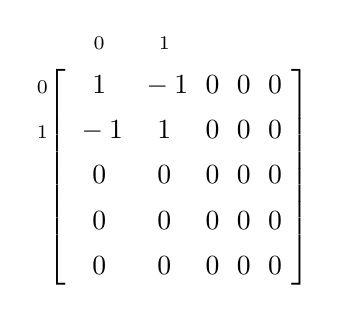
\begin{tikzpicture}[baseline={([yshift=-\dimexpr\fontdimen22\textfont2\relax]M.center)}]
  \matrix [
    matrix of math nodes,
    left delimiter={[}, right delimiter={]},
    inner sep=1pt, column sep=1ex, row sep=1ex,
    execute at begin cell=\mathstrut,
  ] (M) {
    1 & -1 & 0 &  0  &  0 \\
    -1 &  1  & 0 & 0 & 0 \\
    0  &  0  &  0  & 0 &  0  \\
    0  & 0 & 0 &  0  & 0 \\
    0  & 0 &  0  & 0 & 0 \\
  };

	\node[above=1em] at (M-1-1) {$\scriptstyle 0$};
    \node[above=1em] at (M-1-2) {$\scriptstyle 1$};
  
    \node[left=1.5em] at (M-1-1) {$\scriptstyle 0$};
    \node[left=1.5em] at (M-2-1) {$\scriptstyle 1$};

\end{tikzpicture}
\]
\end{document}
